\documentclass[a4j,12pt]{jarticle}


% \usepackage{a4j}
\usepackage{fancyhdr}
\usepackage{lastpage}

% \usepackage{showkeys}
% \usepackage[dvips]{graphicx}

\usepackage{bm}

\usepackage{amsmath}
\usepackage{amsfonts}
\usepackage{amssymb}
\usepackage{slashed}
% \usepackage{mathbbol}  % 数字も白抜きにしてくれる
\usepackage{multirow}  % Tableで複数のセルにまたがるセルを作れる

\usepackage[a4paper,top=2.5cm,bottom=2.5cm,left=2.5cm,right=2.5cm,headsep=10pt]{geometry}
% \usepackage{graphicx}           % tikzで使う graphicxと競合するので排除
% \usepackage[usenames]{color}
% \usepackage[usenames,dvipdfmx]{color}    % optionは同時に指定出来る。
\usepackage[dvipsnames,dvipdfmx]{xcolor}    % optionは同時に指定出来る。


\usepackage[british]{babel}
\input{colordvi.tex}

\usepackage[dvipdfm,colorlinks,pagebackref,pdfusetitle,urlcolor=blue,citecolor=MidnightBlue,linkcolor=MidnightBlue,bookmarksnumbered,plainpages=false]{hyperref}



\input{dummy.tex}

%%% tikzセッティング %%%%%%%%%%%%%%%%%%%%%%%%%%%%%%%
\usepackage[dvipdfmx]{graphicx}
\usepackage{tikz}
\usetikzlibrary{arrows,shapes,patterns,snakes,calc}
\input{arrowsnew}
\usetikzlibrary{decorations.markings}
\usetikzlibrary{positioning}
%%% end of tikz %%%%%%%%%%%%%%%%%%%%%%%%%%%%%%%%%%%%

\usepackage[hang,bf,figurename=Fig.\ , tablename=Table\ ,margin=1cm]{caption}
\renewcommand{\captionfont}{\footnotesize}

%%% listingsセッティング %%%%%%%%%%%%%%%%%%%%%%%%%%%
\usepackage{listings, jlisting}
\renewcommand{\lstlistingname}{Code}
\definecolor{mygreen}{rgb}{0,0.6,0}
\definecolor{mygray}{rgb}{0.5,0.5,0.5}
\definecolor{mymauve}{rgb}{0.58,0,0.82}

\lstset{ %
  % language=Octave,                 % the language of the code
  backgroundcolor=\color{white},   % choose the background color; you must add \usepackage{color} or \usepackage{xcolor}
  basicstyle=\footnotesize,        % the size of the fonts that are used for the code
  breakatwhitespace=false,         % sets if automatic breaks should only happen at whitespace
  breaklines=true,                 % sets automatic line breaking
  captionpos=t,                    % sets the caption-position to bottom
  commentstyle=\color{mygreen},    % comment style
  deletekeywords={...},            % if you want to delete keywords from the given language
  escapeinside={\%*}{*)},          % if you want to add LaTeX within your code
  extendedchars=true,              % lets you use non-ASCII characters; for 8-bits encodings only, does not work with UTF-8
  frame=single,                    % adds a frame around the code
  keepspaces=true,                 % keeps spaces in text, useful for keeping indentation of code (possibly needs columns=flexible)
  keywordstyle=\color{blue},       % keyword style
  morekeywords={*,...},            % if you want to add more keywords to the set
  numbers=left,                    % where to put the line-numbers; possible values are (none, left, right)
  numbersep=5pt,                   % how far the line-numbers are from the code
  numberstyle=\tiny\color{mygray}, % the style that is used for the line-numbers
  rulecolor=\color{black},         % if not set, the frame-color may be changed on line-breaks within not-black text (e.g. comments (green here))
  showspaces=false,                % show spaces everywhere adding particular underscores; it overrides 'showstringspaces'
  showstringspaces=false,          % underline spaces within strings only
  showtabs=false,                  % show tabs within strings adding particular underscores
  stepnumber=1,                    % the step between two line-numbers. If it's 1, each line will be numbered
  stringstyle=\color{mymauve},     % string literal style
  tabsize=2,                       % sets default tabsize to 2 spaces
  title=\lstname                   % show the filename of files included with \lstinputlisting; also try caption instead of title
}
%%% ned of listings セッティング %%%%%%%%%%%%%%%%%%%%%%%%%%%


\pdfstringdefDisableCommands{%
    \renewcommand*{\bm}[1]{#1}%
    % any other necessary redefinitions 
}

%%%今村セッテッティング%%%%%%%%%%%%%%%%%%%%%%%%%%%%%
\newcommand{\CC}{\mathbb{C}}
\newcommand{\ZZ}{\mathbb{Z}}
\newcommand{\RR}{\mathbb{R}}
\newcommand{\HH}{\mathbb{H}}

\newcommand{\hf}{\frac{1}{2}}
\newcommand{\tr}{{\rm tr}}
\newcommand{\ind}{{\rm ind}}
\newcommand{\ol}{\overline}
\newcommand{\ul}{\underline}
\newcommand{\up}{\uparrow}
\newcommand{\dn}{\downarrow}
\newcommand{\wt}{\widetilde}
\newcommand{\ra}{\rightarrow}
\newcommand{\wh}{\widehat}


%%%横山セッティング%%%%%%%%%%%%%%%%%%%%%%%%%%%%%%%%%
\newcommand{\NN}{\mathcal{N}\!}
\newcommand{\DD}{\mathcal{D}}
\newcommand{\UU}{U(1)}
\newcommand{\dd}{\mathrm{d}}
\renewcommand{\SS}{\mathbf{S}}
\renewcommand{\Im}{\mathrm{Im}}
\renewcommand{\Re}{\mathrm{Re}}
\renewcommand{\<}{\langle}
\renewcommand{\>}{\rangle}
\newcommand{\Tr}{{\rm Tr}}

\renewcommand{\r}{\mathrm}

\newcommand{\sign}{\mathrm{sign}}

\newcommand{\lra}{\leftrightarrow}
\newcommand{\LL}{\mathcal{L}}
\newcommand{\la}{\leftarrow}
\newcommand{\ro}{\sqrt}
\newcommand{\Ra}{\Rightarrow}
\newcommand{\Pexp}{\mathrm{Pexp}}

\newcommand{\nn}{\nonumber \\}
\newcommand{\1}{\mbox{1}\hspace{-0.25em}\mbox{l}}

%数字のみ対応
\newcommand{\Maru}[1]{\ooalign{
\ifnum#1<10 \hfil\resizebox{.9\width}{.85\height}{#1}\hfil
\else
\hfil\resizebox{.6\width}{.8\height}{#1}\hfil
\fi
\crcr
\raise.1ex\hbox{$\bigcirc$}}}

%全文字対応
\newcommand{\maru}[1]{\ooalign{
\hfil\resizebox{.8\width}{\height}{#1}\hfil
\crcr
\raise.1ex\hbox{\large$\bigcirc$}}}


\newcommand{\nord}[1]{\vcentcolon\mathrel{#1}\vcentcolon}
\providecommand{\vcentcolon}{\mathrel{\mathop{:}}}


\def\P{\mathop{\cal P}}
\def\diag{\mathop{\rm diag}}


\def\Re{\mathop{\rm Re}\nolimits}
\def\Im{\mathop{\rm Im}\nolimits}
\def\Det{\mathop{\rm Det}\nolimits}
\def\sign{\mathop{\rm sign}\nolimits}


%%% rap %%% - make two letters overlap
\newcommand{\rap}[2]
{\setbox1=\hbox{#1}%
\setbox2=\hbox to\wd1{\hss #2\hss}%
\mbox{\rlap{\box1}\box2}}

%\newcommand{\sla}[1]{\rap{$#1$}{/}}
\newcommand{\sla}[1]{\rap{$#1$}{$\backslash$}}


\def\DY#1{{\MyGreen [DY: #1]}}
\newcommand{\MyGreen}{\color [rgb]{0,0.7,0}}

\usepackage[vcentermath]{youngtab}
% \Yboxdim4pt
\newcommand{\Y}{\yng}
\newcommand{\Young}{}


%%%title def%%%%%%%%%%%%%%%%%%%%%%%%%%%%%%%%%%%%%%%%%%%%%%%

\makeatletter
\def\maketitle{
\noindent
{\Large \@title \par\vskip 2pt}
\noindent
{\large \@date \hspace{4pt} \@author}
%\\[-2pt]
%\noindent------------------------------------------------------------------------------------------
\par\vskip 1.5em
}

\author{横山 大輔}
\date{\today}
%%%本文%%%%%%%%%%%%%%%%%%%%%%%%%%%%%%%%%%%%%%%%%%%%%%%%%%%%%%%%

% \title{\centerline{Lecture 2}}
\begin{document}
% \maketitle
% \begin{abstract}

% \end{abstract}
% \tableofcontents

  \pagestyle{fancy}
  \renewcommand{\headrulewidth}{0.0pt}
  \rhead{}
  \lhead{}
  \cfoot{[\ \scshape\oldstylenums{\thepage}\ / %
    \scshape\oldstylenums{\pageref{lastpage}} ]}
%  \rfoot{\@author}

% \setcounter{section}{}
% \setcounter{subsection}{}
% \setcounter{subsubsection}{}

\centerline{\Large \bf  Lecture 12}

% \vspace{12pt}
% \DY{なにかコメント}

% \vspace{-12pt}

% \vspace{-4pt}
% \begin{itemize}
%  \setlength{\itemsep}{0pt}
%  \item Type I superstring theory.
%  \item In type I theory, we only have D$1$-, D$5$-, and D$9$-, branes.
%  \item O$9^-$-plane is needed for type I to be consistent theory.
%  \item T-duality of type I theory.
% \end{itemize}
% \vspace{-4pt}


\section{Supergravity}

String theory includes massless states as well as massive states.
However, in a low-energy(IR) region, we do not see the stringy massive states 
because the mass $M^2 \sim \frac{1}{\alpha'} \sim \frac{1}{l_s^2}$ is assumed to be very heavy.
Therefore, in the IR limit, we can describe the theory by so called \textbf{effective theory}, 
which only contains the lightest particles(states).
The effective theory, of course, does not contain all the information of the original theory, 
however, it does give us some information of the original theory.


For the bosonic string theory the lightest particles are the massless states (except non-physical tachyon),
and we saw that the effective theory is (Lecture 4)
\begin{align}
 S_\mathrm{eff} = \frac{1}{2\kappa_{26}^2} \int d^{26} X \sqrt{-G} e^{-2\Phi} \left[
 R -\frac{1}{12} H_{\mu\lambda\rho}H^{\mu\lambda\rho}
 +4 \nabla^\lambda\Phi \nabla_\lambda\Phi  \right] \ ,
\end{align}
where $2\kappa_{26}^2$ is a gravitational coupling and it is related to
the Newton constant as $2\kappa_{26}^2 = 16 \pi G_N$.
What we will see below is supersymmetric versions of this,
that are effective theories of IIA/IIB superstring theory and
called type \textbf{IIA/IIB SUGRA} (SUpersymmetric GRAvity).


\subsection{Local SUSY}

Before going to the details of the IIA/IIB SUGRA
let us see general features of SUGRA.

First of all, in order to define spinors in a curved space
we need a vielbein $e_M^a(x^P)$, which transform a local coordinate $x^M$
into a tangent space coordinate (tangent vector) $x^a$ and vice versa (see also Fig.~\ref{tangent.eps}):
\begin{figure}[htb]
\centerline{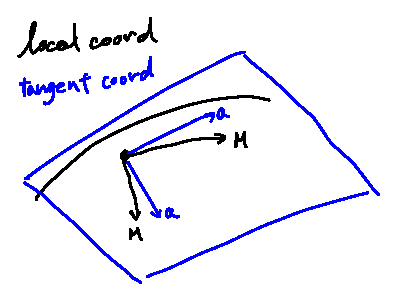
\includegraphics[width=200pt]{tangent.eps}}
\caption{Local coordinate and tangent coordinate.}
\label{tangent.eps}
\end{figure}
\begin{align}
 x^a = e^a_M x^M \ , \quad x^M = e^M_a x^a \ ,
\end{align}
which is defined through space-time metric $G_{MN}$ by
\begin{align}
 G_{MN}(x^P) = \eta_{ab} e_M^a(x^P) e_N^b(x^P)  \ .
\end{align}
Now we can use spinor representations and gamma matrices thanks to the vielbein:
\begin{align}
 \{\Gamma^a,\Gamma^b\} = 2\eta^{ab} \ .
\end{align}



In the case that a theory includes gravity
translation invariance is promoted to general coordinate transformation invariance (the symmetry is localized).
Similarly, global Lorentz symmetry is promoted to local Lorentz symmetry (this is done by the vielbein):
\begin{align}
 \Lambda^a_{\ b} e_a^M(x^P) e_N^b(x^P) \equiv \Lambda^M_{\ N}(x^P) \ .
\end{align}
Gravity is nothing but a gauge field for general coordinate transformation.
In general, gauge field has gauge degrees of freedom
\begin{align}
 \delta A_M = D_M \lambda \ ,
\end{align}
and for gravity it is
\begin{align}
 \delta e_M^a = D_M \lambda^a \ ,
\end{align}
where $\lambda^a$ is a vector gauge transformation parameter, and $D_M$ is a covariant derivative.


Since the translation is promoted to local one
supersymmetry, whose square is roughly translation, should also be promoted to
local supersymmetry.
Correspondingly, there must be a gauge field that transforms with a spinor gauge parameter $\xi^\alpha$ as follows.
\begin{align}
 \delta \psi_M^\alpha = D_M \xi^\alpha \ ,
\end{align}
where $\psi_M^\alpha$ is called Rarita-Schwinger field or \textbf{gravitino}.


SUGRA theory always includes the two gauge fields, $e^a_M$ and $\psi^\alpha_M$,
and their action is given by
\begin{align}
 S = \frac{1}{2\kappa_D^2}\int d^D x\ e\ \left[ R -2i \psi_M \Gamma^{MNP} D_N \psi_P \right] \ ,
\end{align}
where $e = \det e_M^a$, and we omitted the spinor index $\alpha$.
The SUSY transformations for the fields are
\begin{align}
 \delta_\epsilon e^a_M = i\ol\epsilon \Gamma^a \psi_m \ , \qquad
 \delta_\epsilon \psi_M = D_M \epsilon \ .
\end{align}



\subsection{11d SUGRA}

Supersymmetry puts a strong constraint on the dimension of the theory.
If we limit ourselves to consider fields up to spin-$2$,
then, it is known that the highest dimension is $11$.
This is roughly because the D.O.F of fermions grows exponentially: $2^{[D/2]}$,
on the other hand, that of bosons grows as a power of $D$: 
$\frac{(D-1)(D-2)}{2}-1$ (graviton).
Therefore, to balance fermions and bosons we cannot go arbitrary higher.


Although the existence of fermions is crucial,
what we need, to see the connections to string theories,
is the bosonic part.


Let us see the action of the 11d SUGRA.
\begin{align}
 2\kappa_{11}^2 S_{11} = \int d^{11}x \sqrt{ -G} \left[R -\frac{1}{2} K_{(4)}^{2}\right]
 -\frac{1}{6}\int d^{11}x\ M_{(3)} \wedge K_{(4)} \wedge K_{(4)} \ ,
\end{align}
where $K_4 = d M_3$ is a field strength of a rank 3 anti-symmetric tensor $M_3$,
and $K_{(4)}^{2} = K_{(4)} \wedge * K_{(4)}$.
The 11d SUGRA consists of three fields;
one is the graviton $G_{MN}$ (44 states), the other boson is 
rank 3 anti-symmetric tensor $M_{(3)}$ (84 states),
and the gravitino $\psi_M$ (128 states).
We can see that the numbers of fermions and bosons are balanced.
Note that there is only one parameter $\kappa_{11}$,
which can be written in terms of Planck length $l_p$: 
$\frac{1}{2\kappa_{11}^2} = \frac{2\pi}{(2\pi l_p)^9}$.


You may wonder why we looked into such a non-interesting theory
in a sense that what we want is $10$ dimension, rather than $11$ dimension.
One reason is that the interesting $10$d SUGRA can be derived by
dimensional reduction from the $11$ SUGRA.
Other reason, which is rather surprising, will be clear later.


\subsection{10d Type IIA SUGRA}


Let us first write down the action $S_\mathrm{A}$, which is a sum of following three terms.
\begin{align}
 &S_\mathrm{A,NS} = \frac{1}{2\kappa_{10}^2} \int d^{10}x \sqrt{ -G} e^{-2\Phi} \left[
 R +4 \partial_\mu \Phi \partial^\mu \Phi -\frac{1}{2} H_{(3)}^{2} \right] \ ,  \\
 &S_\mathrm{A,R} = \frac{1}{2\kappa_{10}^2} \int d^{10}x \sqrt{ -G} \left[
 -\frac{1}{2} G_{(2)}^{2} -\frac{1}{2} \wt G_{(4)}^{2} \right] \ ,  \\
 &S_\mathrm{A,CS} = -\frac{1}{4\kappa_{10}^2} \int B_{(2)} \wedge G_{(4)} \wedge G_{(4)} \ ,
\end{align}
where $H_{(3)} = dB_{(2)}$, $G_{(2)} = dC_{(1)}$, $\wt G_{(4)} = G_{(4)} -C_{(1)} \wedge H_{(3)}$, $G_{(4)} =dC_{(3)}$,
and $2\kappa_{10}^2 = (2\pi l_s)^8/2\pi$.

The IIA fields are coming from reduction of $11$d SUGRA fields
(the compactified direction is denoted as $\theta$):
\begin{align}
 &G_{MN} \Rightarrow G_{\mu\nu} \ , \quad G_{\mu\theta} \Rightarrow C_1 \ , \quad
 G_{\theta\theta} \Rightarrow \Phi \ ,  \\
 &M_{\mu\nu\theta} \Rightarrow B_{\mu\nu} \ , \quad M_{\mu\nu\rho} \Rightarrow C_{(3)} \ .
\end{align}

In order to see the concrete reduction let us substitute following expression:
\begin{align}
 &ds_{11}^2 = G_{MN} dx^M dx^N = G_{\mu\nu} dx^\mu dx^\nu +l_p^2 e^{2\sigma} (d\theta+C_{(1)})^2 \ , \\
 &M_{(3)} = C_{(3)} +B_{(2)} \wedge d\theta \ , \quad K_{(4)} = \wt G_{(4)} +H_{(3)} \wedge (d\theta +C_{(1)}) \ ,
\end{align}
into the action, and then, the action becomes
\begin{align}
 S_{11} &\Rightarrow \frac{2\pi l_p}{2\kappa_{11}^2}\int d^{10}x \sqrt{ -G} \left[
 e^\sigma R -\frac{1}{2} e^{3\sigma} G_{(2)}^{2} -\frac{1}{2} e^{-\sigma} H_{(3)}^{2}
 -\frac{1}{2} e^{\sigma} \wt G_{(4)}^{2}
 \right] \nn
 &\qquad-\frac{2\pi l_p}{4\kappa_{11}^2}\int d^{11}x\ B_{(2)} \wedge G_{(4)} \wedge G_{(4)} \ .
 \label{eq:1}
\end{align}
Furthermore, we rescale the metric $G_{\mu\nu} = e^{-\sigma} G_{s,\mu\nu}$:
\begin{align}
 \Rightarrow \frac{2\pi l_p}{2\kappa_{11}^2}\int d^{10}x \sqrt{ -G_s} \left[
 e^{-3\sigma} \left(R +9\partial^\mu\sigma\partial_\mu\sigma
 -\frac{1}{2} H_{(3)}^{2} \right)
 -\frac{1}{2} G_{(2)}^{2} -\frac{1}{2} \wt G_{(4)}^{2}
 \right] +\cdots \ .
 % -\frac{2\pi l_p}{4\kappa_{11}^2}\int d^{11}x\ B_2 \wedge G_4 \wedge G_4 \ .
\end{align}
Therefore, we can identify $3\sigma = 2\Phi$.


Let us define $R = l_p e^\sigma$, which is a radius of the compactified circle.
Then, we have following relation.
\begin{align}
 e^{3\sigma} = e^{2\Phi} \quad\Rightarrow\quad \left(\frac{R}{l_p}\right)^3 = g_s^2 \ .
\end{align}
Furthermore, we compare the coupling constant of 11d SUGRA with reduction (\ref{eq:1}) 
and IIA SUGRA:
\begin{align}
 \frac{2\pi R}{2\kappa_{11}^2} = \frac{e^{-2\Phi}}{2\kappa_{10}^2} \quad\Rightarrow\quad
 \frac{2\pi(2\pi R)}{(2\pi l_p)^9} = \frac{2\pi}{g_s^2(2\pi l_p)^8}
 \quad\Rightarrow\quad \frac{R}{l_p^3} = \frac{1}{l_s^2} \ .
\end{align}
Combining the two relation we have $R = g_s l_s$.


\subsection{10d Type IIB SUGRA}


Let us first write down the action $S_\mathrm{B}$, which is a sum of following three terms.
\begin{align}
 &S_\mathrm{B,NS} = \frac{1}{2\kappa_{10}^2} \int d^{10}x \sqrt{ -G}  e^{-2\Phi} \left[
 R +4 \partial_\mu \Phi \partial^\mu \Phi -\frac{1}{2} H_{(3)}^{2} \right] \ ,  \\
 &S_\mathrm{B,R} = \frac{1}{2\kappa_{10}^2} \int d^{10}x \sqrt{ -G} \left[
 -\frac{1}{2} G_{(1)}^{2} -\frac{1}{2} \wt G_{(3)}^{2} -\frac{1}{4} \wt G_{(5)}^{2} \right] \ ,  \\
 &S_\mathrm{B,CS} = -\frac{1}{4\kappa_{10}^2} \int C_{(4)} \wedge H_{(3)} \wedge G_{(3)} \ ,
\end{align}
where $H_{(3)} = dB_{(2)}$, $G_{(1)} = dC_{(0)}$, $G_{(3)} = dC_{(2)}$, $G_{(5)} = dC_{(4)}$, $\wt G_{(3)} = G_{(3)} -C_{(0)} H_{(3)}$, and $\wt G_{(5)} =G_{(5)} -\frac{1}{2}C_{(2)} \wedge H_{(3)} +\frac{1}{2} B_{(2)} \wedge G_{(3)}$.

As we saw in the string theory analysis the string spectrum includes
self-dual 4-form.
The self-dual condition, in the language here, is $* \wt G_{(5)} = \wt G_{(5)}$,
which is different from E.O.M $d*\wt G_{(5)} =0$ or Bianchi id $d \wt G_{(5)} = 0$.
Hence, the condition must be imposed by hand.
This is problematic when you quantize the theory,
however, it is not problem for our purpose.


% \section{Electro-magnetic duality}

% Since we have



\section{String dualities}


In the previous lectures we saw that there exist so called T-duality,
which relates IIA, IIB, and also type I superstring theories.
Although it exchanges the space-time radius $R \lra \wt R = \alpha'/R$
it does not affect coupling constant $g_s$.



Our argument is based on perturbation theory,
which means that the string coupling $g_s$ is small,
otherwise we cannot discuss ``1 string'' states.
Therefore, we do not know what happen in a strong coupling region $g_s >> 1$.
Since the electro-magnetic duality inverse the coupling
we may wonder the same thing could happen in the string theory.



\subsection{S-duality of type IIB SUGRA}

Let us write the action so that we can see the hidden symmetry of the action.
We use $G_{E,\mu\nu} = e^{-\Phi/2} G_{\mu\nu}$, $\tau = C_{(0)} +ie^{-\Phi}$,
\begin{align}
 \mathbb M = \frac{1}{\Im \tau}
 \begin{pmatrix}
  |\tau|^2 & -\Re \tau \\ -\Re \tau & 1
 \end{pmatrix} \ , \qquad
 \mathbb F_{(3)} =
 \begin{pmatrix}
  H_{(3)} \\ G_{(3)}
 \end{pmatrix} \ ,
\end{align}
and the action becomes
\begin{align}
 S_\mathrm{B} = \frac{1}{2\kappa_{10}^2} \int d^{10}x \sqrt{ -G_E} \left[
 R_E - \frac{\partial_\mu \tau \partial^\mu \ol\tau}{2(\Im \tau)^2}
 -\frac{1}{2} \mathbb F_{(3)} \cdot \mathbb M \cdot \mathbb F_{(3)}
 -\frac{1}{4} \wt G_{(5)}^2
 \right]
 -\frac{1}{4\kappa_{10}^2} \int C_{(4)} \wedge \mathbb F_{(3)}^T \wedge \epsilon \mathbb F_{(3)} \ ,
\end{align}
where $\epsilon = \begin{pmatrix} 0 & 1 \\ -1 & 0 \end{pmatrix}$.
This action is invariant under the $SL(2,\mathbb R)$ transformation:
\begin{align}
 \tau' = \frac{a\tau +b}{c\tau +d} \ , \quad
 \mathbb M' = (\Lambda^{-1})^T \mathbb M \Lambda^{-1} \ , \quad
 \mathbb F_{(3)}' = \Lambda \mathbb F_{(3)} \ , \quad
 \Lambda =
 \begin{pmatrix}
  d & c \\ b & a
 \end{pmatrix} \ .
\end{align}
$G_E$ and $C_{(4)}$ are invariant under the transformation.


Let us consider consider D-branes coupled to the RR-fields.
D$3$-brane is invariant because $C_{(4)}$ is invariant.
$5$-branes (NS$5$ and D$5$) are magnetically coupled to 2-form fields ($B_{(2)}$ and $C_{(2)}$),
therefore,
\begin{align}
 \mathbb F_{(3)}' = \Lambda \mathbb F_{(3)} \quad\Rightarrow\quad
 d\mathbb F_{(3)}' =
 \begin{pmatrix}
  J_\mathrm{NS5}' \\ J_\mathrm{D5}'
 \end{pmatrix} =
 \Lambda 
 \begin{pmatrix}
  J_\mathrm{NS5} \\ J_\mathrm{D5}
 \end{pmatrix} \quad\Rightarrow\quad
 \begin{pmatrix}
  \mathrm{NS5}' \\ \mathrm{D5}'
 \end{pmatrix} = \Lambda
 \begin{pmatrix}
  \mathrm{NS5} \\ \mathrm{D5}
 \end{pmatrix} \ .
\end{align}
Strings (F$1$ and D$1$) are electrically coupled to 2-form fields,
hence, have a following action
\begin{align}
 S= \int_\mathrm{F1} B_{(2)} + \int_\mathrm{D1} C_{(2)} +\cdots \ .
\end{align}
this should be invariant, therefore,
\begin{align}
 \begin{pmatrix}
  \mathrm{F1} & \mathrm{D1}
 \end{pmatrix}
 \begin{pmatrix}
  B_{(2)} \\ C_{(2)}
 \end{pmatrix} \quad\Rightarrow\quad
 \begin{pmatrix}
  \mathrm{F1}' & \mathrm{D1}'
 \end{pmatrix} =
 \begin{pmatrix}
  \mathrm{F1} & \mathrm{D1}
 \end{pmatrix} \Lambda^{-1} \quad\Leftarrow\quad
  \begin{pmatrix}
  B_{(2)}' \\ C_{(2)}'
  \end{pmatrix} = \Lambda
  \begin{pmatrix}
  B_{(2)} \\ C_{(2)}
 \end{pmatrix} \ .
\end{align}

Due to the Dirac quantization condition, the electric and the magnetic charges
must be integers, and hence, the true symmetry is $SL(2,\ZZ)$.

In the case of $\Lambda = S =
\begin{pmatrix}
 0 & 1 \\ -1 & 0
\end{pmatrix}$ fields transform
$\tau \lra -1/\tau$, $\mathrm{F1} \lra \mathrm{D1}$, and $\mathrm{NS5} \lra \mathrm{D5}$.
Especially, if $\langle C_0 \rangle = 0$ $g_s \lra 1/g_s$.
Therefore, this is a strong-weak duality !
and typically called \textbf{S-duality}.


Other elements of $SL(2,\ZZ)$ lead
infinitely many bound states of F$1$ and D$1$: $(p,q)$-string,
and those of NS$5$ and D$5$: $(p,q)$ 5-branes.


The argument here implies that IIB superstring theory has also $SL(2,\ZZ)$ symmetry,
and there many evidences for it but there is no proof so far.



\subsection{M-theory}


Since the IIB theory has $SL(2,\ZZ)$ symmetry,
we may expect the similar thing happens in IIA as well.
However, we immediately notice, e.g. that there is no partner for $B_{(2)}$ field, etc.



For IIA superstring theory, rather surprising phenomenon happens
in strong coupling region.
As we saw in the dimensional reduction of 11d SUGRA
we have $R = g_s l_s$.
This means that when we consider strong coupling region another space-time direction
emerges (de-compactification) !!
So far, this deduction is purely from SUGRA analysis, however,
if we assume that the 11d SUGRA is an effective theory of something like ``string''
theory, then, further miraculous coincidence happens.

Witten proposed such a ``string''-like theory and put a name, \textbf{M-theory}.
According to him the M stands for Magic, Mysterious, or Membrane.
Some people also include Matrix, etc. so why not come up with your own M !


Since the 11d SUGRA has 3-form anti-symmetric fields
there must be corresponding objects that coupled to the field electrically and magnetically.
They are called \textbf{M2-brane} and \textbf{M5-brane},
which are $(1+2)$- and $(1+5)$-dimensional objects, respectively.
Let us assume that they have following tensions and charges
\begin{align}
 T_{M2} = \mu_{M2} = \frac{2\pi}{(2\pi l_p)^3} \ , \qquad
 T_{M5} = \mu_{M5} = \frac{2\pi}{(2\pi l_p)^6} \ .
\end{align}

When we put this M-theory on a circle $S^1$, then, it should reduce to
the IIA superstring theory.
Let us see this by comparing the branes and their tensions (see Table~\ref{table:001}).
\begin{table}[htbp]
 \begin{center}
  \caption{Wrapped or unwrapped M-branes and corresponding string and D-branes,
  with their tensions.}
  \vspace{4pt}
  \label{table:001}
\begin{tabular}{c|cccccc}
 Dimension & $0$ & $1$ & $2$ & $4$ & $5$ & $6$ \\
 \hline
 M on $S^1$ & KK-mom. & M2/$S^1$ & M2 & M5/$S^1$ & M5 & KK-mono. \\
 & $\frac{1}{R}$ & $\frac{2\pi\cdot2\pi R}{(2\pi l_p)^3}$ & $\frac{2\pi}{(2\pi l_p)^3}$ & $\frac{2\pi\cdot2\pi R}{(2\pi l_p)^6}$ & $\frac{2\pi}{(2\pi l_p)^6}$ & $\frac{2\pi(2\pi R)^2}{(2\pi l_p)^9}$ \\
 \hline
 IIA & D$0$ & F$1$ & D$2$ & D$4$ & NS$5$ & D$6$ \\
 & $\frac{2\pi}{g_s (2\pi l_s)}$ & $\frac{2\pi}{(2\pi l_s)^2}$ & $\frac{2\pi}{g_s (2\pi l_s)^3}$ & $\frac{2\pi}{g_s (2\pi l_s)^5}$ & $\frac{2\pi}{g_s^2 (2\pi l_s)^6}$ & $\frac{2\pi}{g_s (2\pi l_s)^7}$ \\
\end{tabular}
\end{center}
\end{table}
You should confirm that the tensions perfectly agree.


Note that M-theory is NOT even defined in a sense that we do not know how to quantize
the M-branes.
However, the existence of such a theory tells us a lot.
Especially, even though no effective theory of M$5$-branes in flat space is known,
M$5$-branes wrapped on Riemann manifolds leads amazing relation between
a $d$-dim topological theory and $6-d$ supersymmetric gauge theories
(typical one is M$5$ wrapped on Riemann surface and the relation is called AGT),
which is an ongoing, hot research topic.


\section{D-brane dynamics}

There is so called Dirac-Born-Infeld action, which is an effective action
for D-branes.
It describes motion of the D-branes as well as gauge field living on their world-volume.

Let us consider a simple set up (see Fig.~\ref{D1D2.eps}).
\begin{figure}[htb]
\centerline{\includegraphics[width=250pt]{D1D2.eps}}
\caption{D$1$-brane and its T-dual D$2$-brane.}
\label{D1D2.eps}
\end{figure}
The space-time is $\RR_t \times \RR \times S^1$
and the metric is $ds^2 = \eta_{\mu\nu} dx^\mu dx^\nu$.
D$1$-brane locates at $X_2$ ($\sim X_2 +2\pi R$),
and D$2$-brane has Wilson line $A_2$ ($\sim A_2 +\frac{1}{\wt R}$).
Note that here $A_2$ is not a 2-form but $A_{\mu=2}$.
T-duality relates these quantities (Lecture 9):
\begin{align}
 X_2 = 2\pi \alpha' A_2 \ .
\end{align}
Now consider vibrating D$1$-brane $X^2 = X^2(x^1)$ (see Fig.~\ref{vibD1.eps}).
\begin{figure}[htb]
\centerline{\includegraphics[width=120pt]{vibD1.eps}}
\caption{Vibrating D$1$-brane.}
\label{vibD1.eps}
\end{figure}
It maps to a field strength $F_{12} = \partial_1 X_2(x^1) \neq 0$ on D2-brane.
Suppose the vibrating D$1$-brane is described by Nambu-Goto action
\begin{align}
 S_\textrm{D1} &= -T_\textrm{D1} \int d^2x \sqrt{-\det \left( G_{\mu\nu} \frac{\partial X^\mu}{\partial x^a} \frac{\partial X^\nu}{\partial x^b} \right)} \quad\textrm{with}\quad
 X^0 = x^0 \ , \quad X^1 = x^1 \ , \nn
 &= -T_\textrm{D1} \int dx^0 dx^1 \sqrt{1 +\left(\frac{\partial X^2}{\partial x^1} \right)^2} \ .
\end{align}
This expression seems to coincide with
\begin{align}
 S_\textrm{D2} &= -T_\textrm{D2} \int d^3x \sqrt{-\det \left( G_{\mu\nu} \frac{\partial X^\mu}{\partial x^a} \frac{\partial X^\nu}{\partial x^b} +2\pi \alpha' F_{ab} \right)}  \nn
 &= -T_\textrm{D2} \cdot 2\pi \wt R\cdot \int dx^0 dx^1 \sqrt{1 +\left(2\pi\alpha'F_{12} \right)^2} \ .
\end{align}


From the dimension analysis D-brane tension should be the following form.
\begin{align}
 T_{\mathrm Dp} \sim \frac{\mathrm{mass}}{p\textrm{-dim vol}} \quad\Rightarrow\quad
 T_{\mathrm Dp} \sim \frac{1}{l_s^{p+1}} \ .
\end{align}
From the argument above in order for the two action to coincide
we need $T_\textrm{D1} = 2\pi \wt R T_\textrm{D2}$.
On the other hand, we do not want $T_{\textrm{D}p}$ to depend on $R$ because
$T_{\textrm{D}p}$ should be independent of space-time geometry.
Note that D-brane effective theory is supposed to reproduce open string amplitude,
whose leading contribution is the disk amplitude $\sim e^{-\langle \Phi \rangle}$.
Thus, we propose
\begin{align}
 S_{\textrm{D}p} &= -T_{\textrm{D}p} \int d^{p+1}x e^{-\Phi(X)} \sqrt{-\det \left( G_{\mu\nu}
 \partial_a X^\mu \partial_b X^\nu +2\pi \alpha' F_{ab} \right)} \ .
\end{align}
Then, the ration of effective tension is
\begin{align}
 \frac{T_{\textrm{D}1}^\mathrm{eff}}{T_{\textrm{D}2}^\mathrm{eff}}
 = \frac{T_{\textrm{D}1} e^{-\Phi}}{T_{\textrm{D}2} e^{-\wt\Phi}}
 =  \frac{T_{\textrm{D}1}}{T_{\textrm{D}2}} \cdot \frac{\wt R}{l_s} = 2\pi \wt R
 \quad\Rightarrow\quad T_{\textrm{D}1} = 2\pi l_s \cdot T_{\textrm{D}2} \ .
\end{align}
Note that the dilation field transforms under T-duality as $e^{-\wt\Phi} = e^{-\Phi} \frac{\wt R}{l_s}$.
For D-branes in superstring theory the correct normalization is
$T_{\textrm{D}p} = \frac{2\pi}{(2\pi l_s)^{p+1}}$.



We heavily used the fact that D$p$-branes couples to $C_{p+1}$.
Let us consider a concrete coupling.
It should be the following form.
\begin{align}
 S_{\textrm{D}p} = \cdots + \mu_{\textrm{D}p} \cdot \int d^{p+1}x e^{-\Phi}
 C_{\mu_1\cdots\mu_{p+1}}(X) \frac{\partial X^{\mu_1}}{\partial x^1 } \cdots
 \frac{\partial X^{\mu_{p+1}}}{\partial x^{p+1} }
 = \cdots +\mu_{\textrm{D}p} \cdot \int_{\textrm{D}p} e^{-\Phi} C_{(p+1)} \ .
\end{align}
By considering T-duality we can conclude that
$\mu_{\textrm{D}p} = \frac{2\pi}{(2\pi l_s)^{p+1}} = T_{\textrm{D}p}$ (up to a constant).
Note that we have to use proper normalization of the RR-fields,
depending on the context, which either string analysis or SUGRA analysis.
The convention above is for string analysis.
For SUGRA analysis it is (called canonically normalized one)
\begin{align}
 S_{\textrm{D}p} =
 \cdots +\mu_{\textrm{D}p} \cdot \int_{\textrm{D}p} C_{(p+1)} \ .
\end{align}




Let us again vibrating D$1$-brane with the RR-coupling.
T-duality connects the following two expression.
\begin{align}
 &S_{\textrm{D}1} =
 \cdots +\mu_{\textrm{D}1} \cdot \int dx^0 dx^1 e^{-\Phi}
 \left( C_{01} +C_{02} \frac{\partial X^2}{x^1}\right) \ , \\
 &S_{\textrm{D}2} =
 \cdots +\mu_{\textrm{D}2} \cdot \int dx^0 dx^1 dx^2 e^{-\wt \Phi}
 \left( \wt C_{012} +\wt C_{0} \cdot s\pi\alpha' F_{12} \right) \ ,
\end{align}
where $C_{01} \lra \wt C_{012}$, $C_{02} \lra \wt C_{0}$, and $X^2 \lra 2\pi\alpha' A_2$.
This can be understood as follows (see Fig.).
\begin{figure}[htb]
\centerline{\includegraphics[width=250pt]{D0D2.eps}}
\caption{D$0$-D$0$ bound state.}
\label{D0D2.eps}
\end{figure}
The vibrating D$1$-brane consists of straight D$1$-brane along $x^1$
and local vibration along $x^2$.
After T-duality along $x^2$ the vibration part becomes D$0$-brane and gives
$F_{12}\neq 0$.
Generalization of the RR-coupling is
\begin{align}
 S_{\textrm{D}p} =
 \cdots +\mu_{\textrm{D}p} \cdot \int C_{RR} \wedge \exp(2\pi\alpha' F_{(2)}) \ ,
\end{align}
where $C_{RR} = \sum_{n} C_{(n)}$.


Finally, full general form of D$p$-brane action is given as follows.
\begin{align}
 S_{\textrm{D}p} &= -T_{\textrm{D}p} \int d^{p+1}x e^{-\Phi(X)} \sqrt{-\det \left( G_{ab}
 +2\pi \alpha' F_{ab} -B_{ab} \right)} \nn
 &\qquad +\mu_{\textrm{D}p} \cdot \int C_{RR} \wedge \exp(2\pi\alpha' F_{(2)}-B_{(2)}) \ ,
\end{align}
where $G_{ab} = G_{\mu\nu} \partial_a X^\mu \partial_b X^\nu$ and
$B_{ab} = B_{\mu\nu} \partial_a X^\mu \partial_b X^\nu$.


\vspace{12pt}
\noindent
\textbf{Dirac quantization condition}


% Let us consider D$p$-brane located at $\bm x_{\perp} = (x_{p+1},\cdots,x_9) = \bm 0$.
% Then, the RR-coupling becomes
% \begin{align}
%  \mu_{\textrm{D}p} \cdot \int_{\bm x_{\perp} = \bm 0} C_{p+1}
%  = \mu_{\textrm{D}p} \cdot \int_{\bm x_{\perp} = \bm 0} C_{p+1} \wedge \delta(\bm x_{\perp})
%  dx^{p+1} \cdots dx^9 \ .
% \end{align}
% With the kinetic term the action is
% \begin{align}
%  S = -\frac{1}{4\kappa_{10}^2} \int F_{(p+2)} \wedge * F_{(p+2)}
%  +\mu_{\textrm{D}p} \int C_{p+1} \wedge \delta(\bm x_{\perp})
%  dx^{p+1} \cdots dx^9 \ ,
% \end{align}
% and the E.O.M is
% \begin{align}
%  d*F_{(p+2)} = 2\kappa_{10}^2 \mu_{\textrm{D}p} \delta(\bm x_{\perp})
%  dx^{p+1} \cdots dx^9 \ .
% \end{align}
% Integration over ball that perpendicular to the world-line of the D$p$-brane leads
% \begin{align}
%  2\kappa_{10}^2 \mu_{\textrm{D}p} = 
% \end{align}


Let us consider a $(p+1)$-form RR field.
The electrically coupled object is D$p$-brane and the magnetic one is D$(6-p)$-brane.
The magnetic charge of the D$(6-p)$-brane is
\begin{align}
 \mu_{6-p} = \frac{1}{2\kappa_{10}^2} \int_{B^{p+3}} d F_{(p+2)} =
 \frac{1}{2\kappa_{10}^2} \int_{\partial B^{p+3}} F_{(p+2)} \ .
\end{align}
Now consider D$p$-brane moving around D$(6-p)$-brane.
\begin{align}
 S \sim \mu_{p} \int_M C_{(p+1)} = \mu_{p} \int_{\partial^{-1}M} F_{(p+2)} \ ,
\end{align}
where $\partial^{-1}M$ is manifolds whose boundary is $M$.
The choice of $\partial^{-1}M$ is arbitrary, and does not affect the result.
Consider $\partial^{-1}M_N -\partial^{-1}M_S$ surround the D$(6-p)$-brane.
\begin{align}
 \mu_{p} \int_{\partial^{-1}M_N} F_{(p+2)} -\mu_{p} \int_{\partial^{-1}M_S} F_{(p+2)}
 = \mu_{p} \mu_{6-p} 2\kappa_{10}^2 \in 2\pi \ZZ \ .
\end{align}
The values $\mu_{p} = \frac{2\pi}{(2\pi l_s)^{p+1}}$,
$2\kappa_{10}^2 = \frac{(2\pi l_s)^{8}}{2\pi}$ satisfy the quantization condition.



Assume the condition works also for F$1$-string and NS$5$-brane,
\begin{align}
 T_\mathrm{F1} \cdot T_\mathrm{NS5} \cdot 2\kappa_{10}^2 g_s^2 = 2\pi \ ,
\end{align}
where we are in the string frame.
Since $T_\mathrm{F1} = \frac{2\pi}{(2\pi l_s)^2}$,
\begin{align}
 T_\mathrm{NS5} = \frac{2\pi}{T_\mathrm{F1} \cdot 2\kappa_{10}^2 g_s^2}
 = \frac{2\pi}{(2\pi l_s)^6 g_s^2} \ .
\end{align}


















  

% \begin{thebibliography}{CDLOGP91}

%  \bibitem[Pol98]{Pol98}
%                 J. Polchinski.
%                 String theory. Vol. 1.
%                 Cambridge University Press, 1998.

%  \bibitem[BP09]{Blumenhagen:2009zz}
%                R.~Blumenhagen and E.~Plauschinn.
%                \newblock {Introduction to conformal field theory}.
%                \newblock {\em Lect. Notes Phys.}, 779:1--256, 2009.

% \end{thebibliography}


% \bibliography{string-lecture}
% \bibliographystyle{halpha}
% \bibliographystyle{JHEP}

% \begin{thebibliography}{CDLOGP91}

% %\cite{AlvarezGaume:1981hn}
% \bibitem[AFM81]{AlvarezGaume:1981hn}
%   L.~Alvarez-Gaume, D.~Z.~Freedman and S.~Mukhi,
%   ``The Background Field Method and the Ultraviolet Structure of the Supersymmetric Nonlinear Sigma Model,''
%   Annals Phys.\  {\bf 134}, 85 (1981).
%   %doi:10.1016/0003-4916(81)90006-3
%   %%CITATION = doi:10.1016/0003-4916(81)90006-3;%%
%   %525 citations counted in INSPIRE as of 09 Oct 2017



% \bibitem[CT88]{Callan:1988xx}
%  Curt Callan and Lárus Thorlacius.
%  \textit{SIGMA MODELS AND STRING THEORY.}
%  TASI Lecture, 1988.
%  (The link below is a direct link to the pdf file of 45MB )
%  \href{http://www.damtp.cam.ac.uk/user/tong/string/sigma.pdf}
%  {http://www.damtp.cam.ac.uk/user/tong/string/sigma.pdf}.




% \end{thebibliography}


\label{lastpage}

% \begin{tikzpicture}[>=stealth,scale=1]
%  \draw[->] (0,0)--(1,0);
%  \draw[latex-stealth] (0,0.5)--(1,0.5);
%  \draw[latex-stealthnew,arrowhead=2mm] (0,1)--(1,1);
% \end{tikzpicture}

% \begin{figure}[htb]
% \centerline{\includegraphics[width=250pt]{.eps}}
% \caption{}
% \label{.eps}
% \end{figure}



% \begin{table}[htbp]
%  \begin{center}
%   \caption{}
%   \vspace{4pt}
%   \label{table:001}
% \begin{tabular}{|c|c|c|c|c|}
% \hline
% \hline
%   Category & Sector & $(h_A,h_B,h_T)$ & Mirror theory & ABJM model \\
% \hline
%  1 & & \parbox{40pt}{$(0,0,0)$ $(1,1,1)$} & $1.11906$ & $1.13290$ \\
% \hline
%  2 & & \parbox{40pt}{$(0,0,1)$ $(1,1,0)$} & $-0.10861$ & $-0.10861$ \\
% \hline
%  \multirow{2}{*}{\vspace{-15pt}3} & 3-1 & \parbox{40pt}{$(0,1,0)$ $(1,0,1)$} & $0.176777$ &
%  \multirow{2}{*}{\vspace{-15pt}$0.176577$} \\
% \cline{2-4}
%  & 3-2 & \parbox{40pt}{$(1,0,0)$ $(0,1,1)$} & $0.176777$ & \\
% \hline
% \hline
% \end{tabular}
% \end{center}
% \end{table}


% \begin{thebibliography}{99}

% % \cite{Imamura:2012rq}
% \bibitem{Imamura:2012rq}
%   Y.~Imamura and D.~Yokoyama,
%   %``S^3/Z_n partition function and dualities,''
%   JHEP {\bf 1211}, 122 (2012)
%   [arXiv:1208.1404 [hep-th]].
%   %%CITATION = ARXIV:1208.1404;%%

 % \bibitem{fnorio:legendre}
 %         fnorio
 %         ``ルジャンドル変換とは何か''
 %         \url{http://fnorio.com/0146Legendre_transformation/Legendre_transformation.html}


 % \bibitem{EMAN:dynamics}
 %         EMAN物理学
 %         ``ハミルトニアン''
 %         \url{http://eman-physics.net/analytic/hamilton.html}


 % \bibitem{Wiki:legendre}
 %         Wiki
 %         ``ルジャンドル変換''
 %         \url{https://ja.wikipedia.org/wiki/ルジャンドル変換}

 % \bibitem{mathtrain:legendre}
 %         高校数学の美しい物語
 %         ``ルジャンドル変換の意味と具体例''
 %         \url{http://mathtrain.jp/legendrehenkan}

% \end{thebibliography}


% \bibliography{dd}

\end{document}
